%%%%%%%%%%%%%%%%%%%%%%%%%%%%%%%%%%%%%%%%%
% fphw Assignment
% LaTeX Template
% Version 1.0 (27/04/2019)
%
% This template originates from:
% https://www.LaTeXTemplates.com
%
% Authors:
% Class by Felipe Portales-Oliva (f.portales.oliva@gmail.com) with template 
% content and modifications by Vel (vel@LaTeXTemplates.com)
%
% Template (this file) License:
% CC BY-NC-SA 3.0 (http://creativecommons.org/licenses/by-nc-sa/3.0/)
%
%%%%%%%%%%%%%%%%%%%%%%%%%%%%%%%%%%%%%%%%%

%----------------------------------------------------------------------------------------
%	PACKAGES AND OTHER DOCUMENT CONFIGURATIONS
%----------------------------------------------------------------------------------------

\documentclass[
	12pt, % Default font size, values between 10pt-12pt are allowed
	%letterpaper, % Uncomment for US letter paper size
	%spanish, % Uncomment for Spanish
]{fphw}

% Template-specific packages
\usepackage[utf8]{inputenc} % Required for inputting international characters
\usepackage[T1]{fontenc} % Output font encoding for international characters
\usepackage{mathpazo} % Use the Palatino font

\usepackage{graphicx} % Required for including images

\usepackage{booktabs} % Required for better horizontal rules in tables

\usepackage{listings} % Required for insertion of code

\usepackage{enumerate} % To modify the enumerate environment

\usepackage{hyperref}

%----------------------------------------------------------------------------------------
%	ASSIGNMENT INFORMATION
%----------------------------------------------------------------------------------------

\title{Homework \#2} % Assignment title

\author{ } % Student name

\date{ January 24th, 2024} % Due date

\institute{The \textit{Abdus Salam} International Centre for Theoretical Physics \\ Master of Advanced Studies in Medical Physics} % Institute or school name

\class{2024 Statistics for Medicine} % Course or class name

\professor{Massimo Borelli} % Professor or teacher in charge of the assignment

%---------------------------------------

\begin{document}

\maketitle % Output the assignment title, created automatically using the information in the custom commands above

%----------------------------------------
%	ASSIGNMENT CONTENT
%----------------------------------------
\section*{Question}

 \begin{center}
	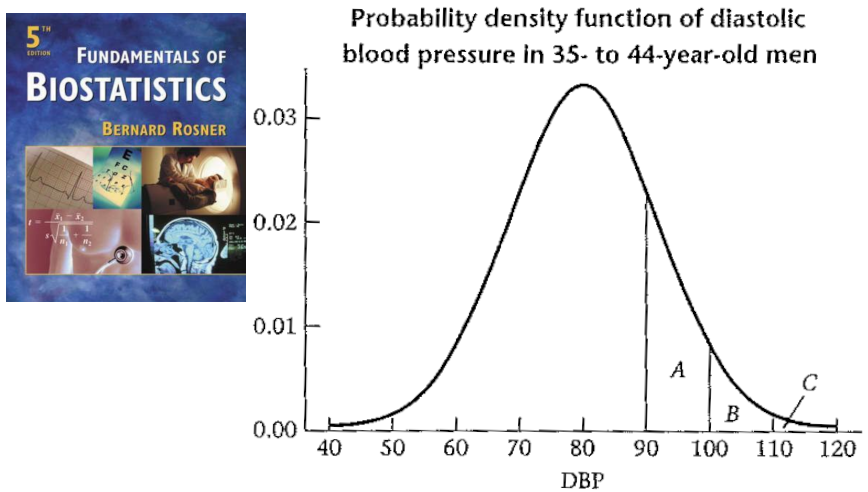
\includegraphics[width=0.55\columnwidth]{02diastolic.png} % Example image
 \end{center}



\begin{problem}

1. Refer to the above graph as proposed by Bernard Rosner, concerning the normally distributed diastolic blood pressure. \\
 
2. (Integration) Evaluate by means of \textsf{JASP} the probabilities of region \textit{A}, \textit{B} and \textit{C}.\\

\end{problem}


\begin{problem}


3. (Not compulsory - optional for experienced students) \textbf{the Monte Carlo methods}. Simulate 10000 normally distributed random point to replicate the above graph, and numerically compute the estimates for \textit{A}, \textit{B} and \textit{C}. Verify the equivalence of findings. \\

\end{problem}


\begin{problem}

4. Report the 2. (and optionally the 3.) outputs, eventually arranged in a more readable form, into the \textbf{Answer} section of the present Homework \# 2. \\

5. Go to \url{https://forms.gle/GotQxrQuaDMyLKps6} in order to upload your final .pdf document.


\end{problem}


%-----------------------------------------

\subsection*{Answer}



% ------  Please, provide an answer ----


% ------  Please, remember to complete the 49 line, "author" section with your Name and Surnale ----



%---------------------------------------

\end{document}
